\documentclass[a4paper,10pt,twoside]{article}

\title{Software for synthesis of function generators cam-follower systems for rapid prototyping}
\author{Federico Ciotti}
\date{December 2016}

\usepackage[T1]{fontenc}
\usepackage[utf8]{inputenc}
\usepackage[english]{babel}
\usepackage{helvet}
\renewcommand{\familydefault}{\sfdefault}
%\renewcommand{\normalsize}{\fontsize{10}{13}\selectfont}
% \setlength{\baselineskip}{1.3em}
%\renewcommand{\baselinestretch}{1.1}
\usepackage{graphicx}
\usepackage{color}
\definecolor{sapienza}{RGB}{130,36,51}
\usepackage{sectsty}
\usepackage[compact]{titlesec}
%\titlespacing*{\section}{0pt}{0.5\baselineskip}{0pt}
\allsectionsfont{\bfseries\normalsize}
\usepackage{geometry}
\usepackage{listings}
\usepackage{minted}

%\let\oldvrb\verbatim
%\renewenvironment{verbatim}{\begin{small}\begin{oldvrb}}{\end{oldvrb}\end{small}}

%\let\oldminted\minted
%\renewenvironment{minted}{\begin{oldminted}{python}}{\end{oldminted}}

%\newenvironment{python}{\begin{pycode}}{\end{pycode}}

\usepackage{fancyhdr}
\setlength{\headheight}{3.65cm}
\pagestyle{fancy}
\fancyhf{}
\lhead{\resizebox{6cm}{!}{
\includegraphics{header}}}
\cfoot{\thepage}
\renewcommand{\headrulewidth}{0pt}
\fancypagestyle{first}{\cfoot{}}

\setlength{\parindent}{0pt}
\setlength{\parskip}{0.4em}

\newminted[pycode]{python}{autogobble}
\newmintedfile[py]{python}{fontsize=\footnotesize}

\begin{document}
\lstset{language=Python}
\newgeometry{includeheadfoot,top=1.25cm,bottom=1.25cm,left=4.5cm,right=3.5cm}
\makeatletter
\begin{titlepage}
    \thispagestyle{first}

    \begin{center}
        \large{\textcolor{sapienza}{Elaborato finale per il conseguimento\\della Laurea in Ingegneria meccanica}}\par
        \vspace{1.2cm}
        {\Large\textbf{\@title}}\par
        \vspace{0.6cm}
        \begin{itshape}
        \large{Candidato: \@author
        \\Matricola: 1593763}\par
        \vspace{1cm}
        Relatore: prof. Nicola Pio Belfiore
        \\SSD: ING-IND/13\par
        \end{itshape}
        \vspace{1cm}
    \end{center}

    \textbf{Abstract.} The aim of this project is the development of an open source software for the design of cam-follower
    mechanisms assigned the function of the follower travel or a set of heights to be linked with a given interpolation method.
    The software is addressed to research and rapid prototyping, thus is provided the option of exporting the result as
    collection of points in CSV form or directly as tridimensional STL model.\par
    \bigskip
    Lo scopo di questo progetto è lo sviluppo di un software open source per la progettazione di meccanismi a camma
    assegnata la funzione del movimento traslante della punteria ovvero un insieme di alzate da collegare
    tramite un'interpolazione assegnata. Il software è indirizzato alla ricerca ed alla prototipazione rapida, pertanto si
    è prevista la possibilità di esportare il risultato sotto forma di collezione di punti in formato CSV o direttamente
    come modello tridimensionale in formato STL.
\end{titlepage}
\makeatother

\newgeometry{includeheadfoot,tmargin=1.25cm,bmargin=1.25cm,lmargin=3cm,rmargin=2cm}

\section{Introduction}
    The program interface is an interactive console written in \emph{Python 3} and it makes use of different libraries:

    \begin{itemize}\itemsep0em
        \item
          \emph{numpy} for array processing
        \item
          \emph{matplotlib} for plotting
        \item
          \emph{shapely} for geometric analysis
        \item
          \emph{scipy} for interpolation
        \item
          \emph{sympy} for expression parsing
        \item
          \emph{pyclipper} for polygon offsetting
        \item
          \emph{stl} for stl manipulation
    \end{itemize}

\section{Usage}
    Command parsing relies on \emph{argparse} module, which takes charge of
    help generation, so every command's documentation may be requested with
    \texttt{-h} or \texttt{-\/-help} option. Avalaible command are listed here:

    \begin{verbatim}
    usage: {help,exit,gen,update,load,save,draw,export,sim} ...

    positional arguments:
      {help,exit,gen,update,load,save,draw,export,sim}
        help                show this help message
        gen                 generate, unspecified variables set to default
        update              update, unspecified variables unmodified
        load                load from file
        save                save to file
        draw                plot representation
        export              export stl model
        sim                 dynamic simulation
    \end{verbatim}

    \texttt{gen} (and \texttt{update}), \texttt{export} and \texttt{sim} are
    discussed thoroughly in the following sections.

\section{Follower travel generation}
    \begin{verbatim}
    usage: gen travel [-h] [-k {spline,linear,harmonic,cycloidal,parabolic,polynomial}]
                      [--order O] [-n N] [--steps S] [--x0 X0] [--x1 X1]
                      (--input IN | --function F)

    optional arguments:
      -h, --help            show this help message and exit
      -k {spline,linear,harmonic,cycloidal,parabolic,polynomial}
                            kind of interpolation (default: linear)
      --order O, -o O       spline/polynomial order (default: 3)
      -n N                  repetitions per cycle (default: 1)
      --steps S, -s S       interpolation steps (default: 10000)
      --x0 X0, -a X0        lower bound of function evaluation (default: 0)
      --x1 X1, -b X1        upper bound of function evaluation (default: 1)
      --input IN, -i IN     input file (default: None)
      --function F, -f F    function of x (default: None)
    \end{verbatim}

    The travel is generated as discretization of a function between given bounds or
    from interpolation of points from an input file (list of semicolon-separated fraction of unit length and heigth)
    with a given method.

    In the first case the function argument is parsed with \emph{sympify} into
    a \emph{SymPy} expression; is converted into a lambda function; and it is discretized:

    \begin{pycode}
    f = lambdify(x, sympify(f), modules="numpy")
    x = np.linspace(x0, x1, num=steps)
    y = f(x)
    \end{pycode}

    In the second case it is called the appropriate method from the \emph{interpolation} module;
    in linear and spline interpolation are used methods of \emph{scipy.interpolate} that
    compute the whole set of points and return the interpolating function, which is then sampled:

    \begin{pycode}
    # Linear
    f = interpolate.interp1d(xpoints, ypoints)
    x = np.linspace(0, 1, steps)
    y = f(x)

    # Spline
    tck = interpolate.splrep(xpoints, ypoints, k=order, per=True)
    x = np.linspace(0, 1, steps)
    y = interpolate.splev(x, tck)
    \end{pycode}

    In harmonic, cycloidal, parabolic and polynomial interpolation a linking function is found
    for every couple of consecutive points:

    \begin{pycode}
    # Harmonic
    x = np.linspace(x0, x1, steps)
    y = y0 + (y1-y0)/2*(1-np.cos(np.divide(np.pi*(x+(-x0)), x1-x0)))
    
    # Cycloidal
    x = np.linspace(x0, x1, steps)
    r = np.divide(x+(-x0), x1-x0)
    y = y0 + (y1-y0)/np.pi*(np.pi*r-np.sin(2*np.pi*r)/2)
    
    # Parabolic
    x = np.linspace(x0, (x0+x1)/2, steps)
    r = np.divide(x + (-x0), x1 - x0)
    y = y0 + 2*(y1-y0)*r**2
    x2 = np.linspace((x0+x1)/2, x1, steps)
    r2 = np.divide(x2 + (-x0), x1 - x0)
    y2 = y0 + (y1-y0)*(1-2*(1-r2)**2)
    
    # Polynomial, solve Vandermonde matrix with added rows for conditions on derivatives
    A = np.zeros((2+order*2, 2+order*2))
    B = np.zeros(2+order*2)
    B[0] = 0
    B[1] = y1-y0
    for col in range(0, 2+order*2):
        A[0, col] = 0 ** col
        A[1, col] = (x1-x0) ** col
    for deriv in range(1, order + 1):
        B[deriv*2] = 0
        B[1+deriv*2] = 0
        for col in range(0, 2+order*2):
            # method der(x,n,k) returns the k-th derivative of x^n
            A[deriv*2, col] = der(0, col, deriv)
            A[1+deriv*2, col] = der((x1-x0), col, deriv)
    c = np.linalg.solve(A, B)
    x = np.linspace(0, x1-x0, steps)
    y = np.polyval(c[::-1], x)
    \end{pycode}

    The result is kept in memory in the arrays \emph{x} and \emph{y} of a persistent
    instance of the class \emph{Travel}.

    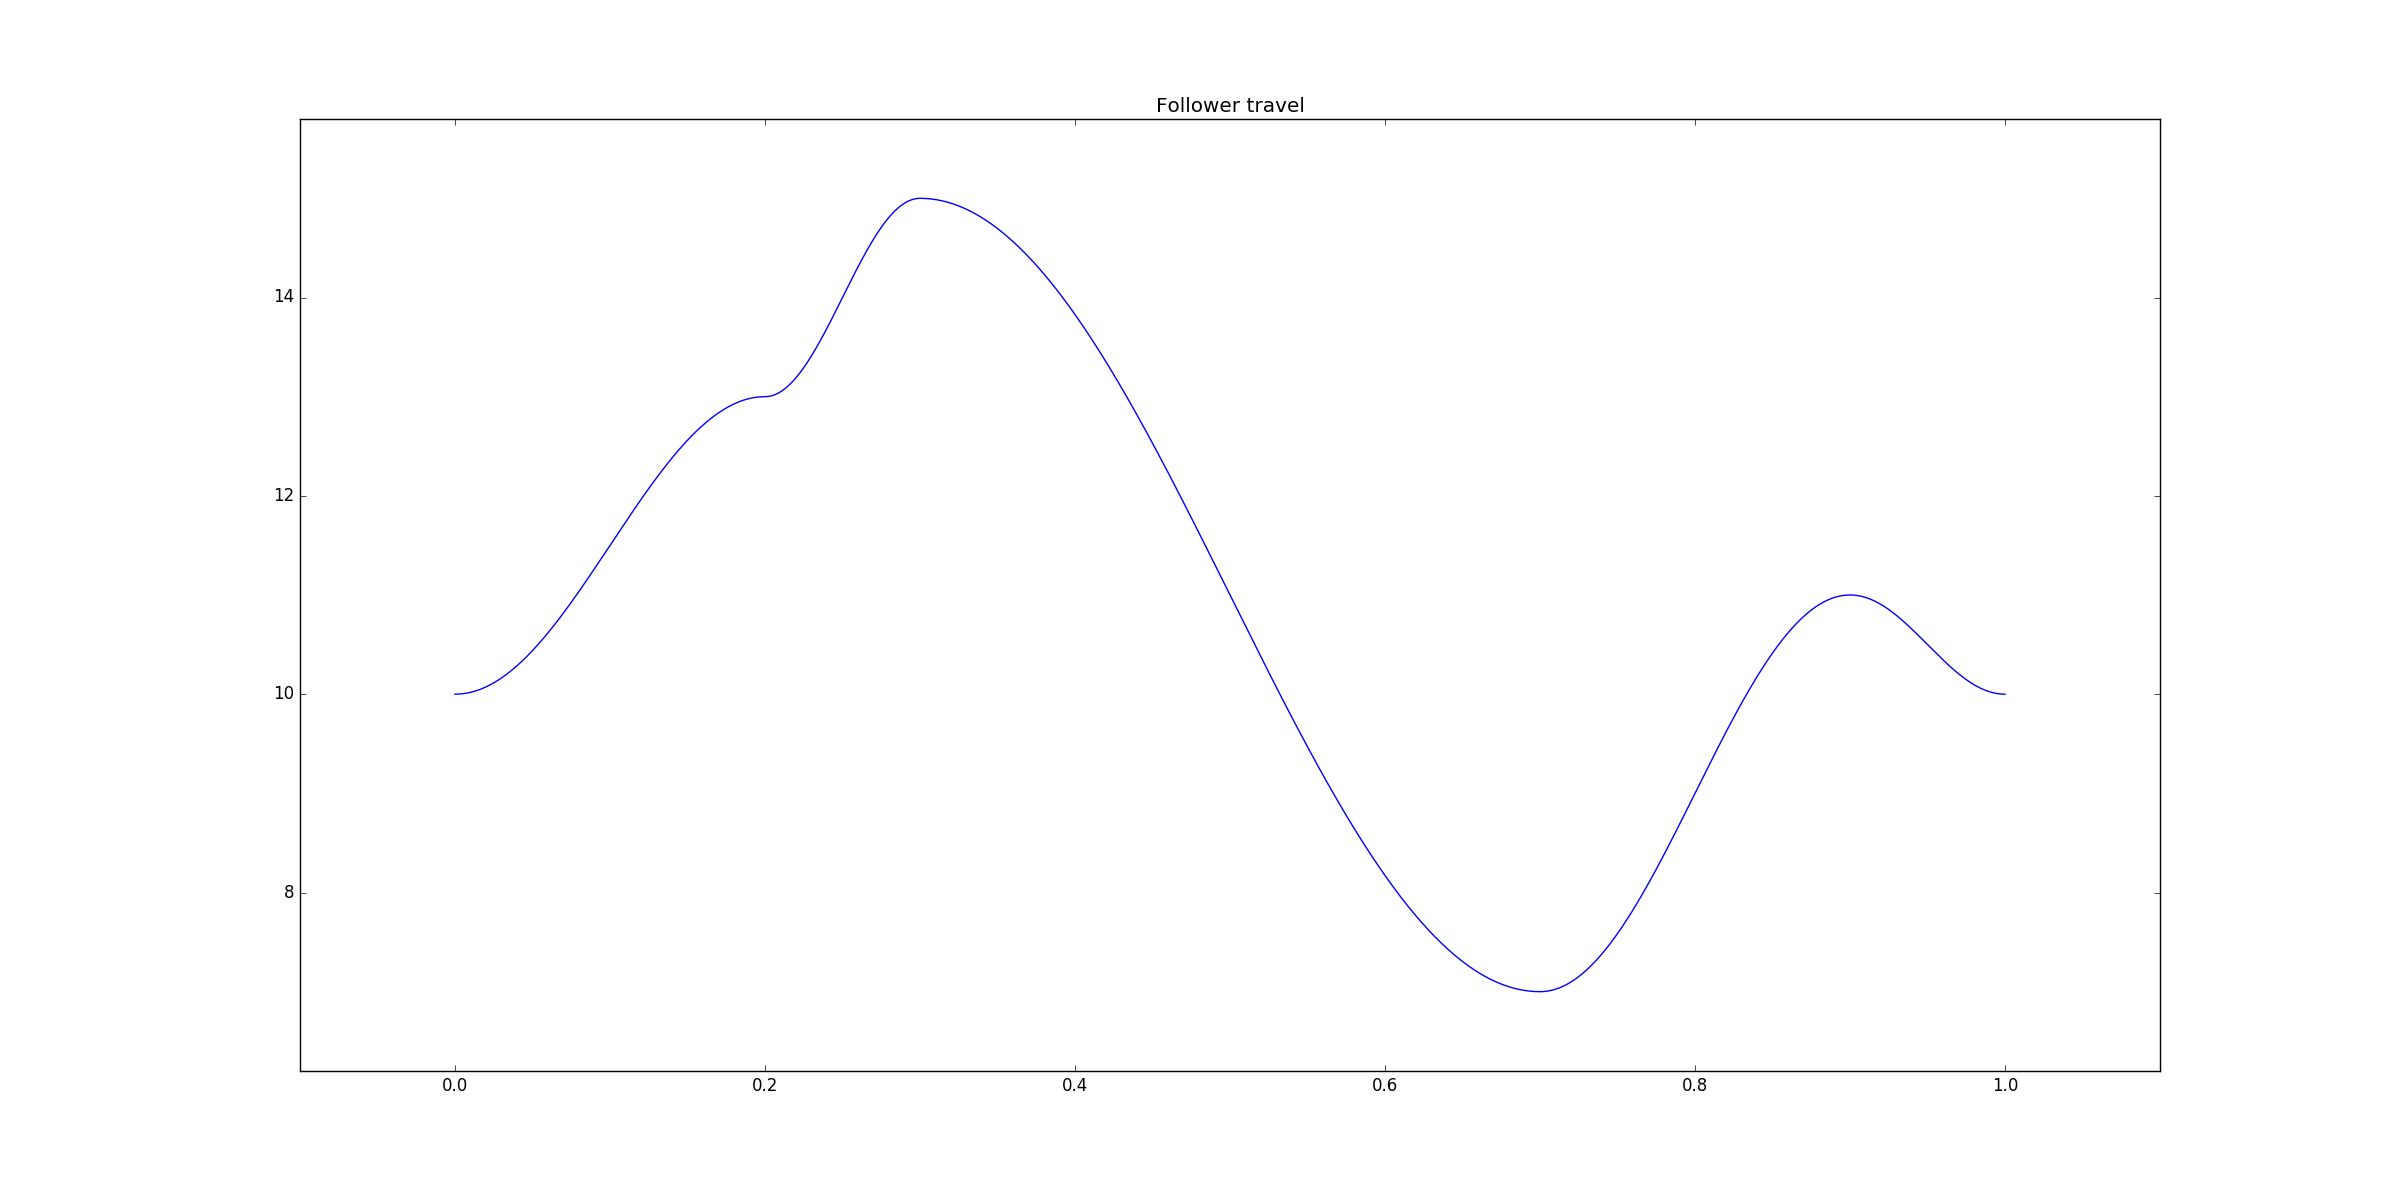
\includegraphics[width=\textwidth]{travel.png}

\section{Cam generation}
    \begin{verbatim}
    usage: gen cam [-h] [--radius R] [--ccw] [--flat] [--offset OFF] [--fradius R]

    optional arguments:
      -h, --help            show this help message and exit
      --radius R, -r R      base radius (default: 0)
      --ccw                 counterclockwise (default: False)
      --flat, -f            flat follower (default: False)
      --offset OFF, -d OFF  follower offset (default: 0)
      --fradius R, -q R     follower radius (set 0 for knife edge) (default: 0)
    \end{verbatim}

    The cam is generated from the travel saved in memory.
    The class \emph{Cam} distinguishes the follower kind and calls the appropriate methods.
    In case of a knife follower the cam profile is generated immediately, else an appropriate method is called.

    \begin{pycode}
    if follower.kind == 'knife':
        if follower.offset == 0:
            pcoords[1] = travel.y + radius
        else:
            pcoords[1] = np.sqrt(follower.offset**2+(radius+travel.y)**2)
    elif follower.kind == 'roller':
        if follower.offset == 0:
            pcoords[1] = travel.y + radius - follower.radius
        else:
            rho_trace = np.sqrt(follower.offset ** 2 + (radius + travel.y) ** 2)
            pcoords = envelope.roller(pcoords[0], rho_trace, follower.radius)
    elif follower.kind == 'flat':
        pcoords = envelope.flat(np.array([pcoords[0], travel.y + radius]))
    if ccw:
        pcoords[1] = pcoords[1][::-1]
    \end{pycode}

    In the pseudo-envelope of flat follower the program, for each point of the pitch curve,
    calculates the distances of intersection of the lines passing through every other point
    and perpendicular to the line connecting the point to the origin \((\perp \theta)\)
    and takes the smallest positive one as value of \(\rho\) in the point direction \(\theta_0\).

    The roller follower envelope is done by offsetting of follower radius the polygonal pitch curve.
    For it is used Pyclipper, a wrapper of Clipper library, which only computes integers,
    so a scaling preserving a good precision is needed. Here is used a factor that sets the precision to
    the maximum error \(\epsilon\) of the polygonial representation of a circle with radius equal to
    the maximum picth curve's \(\rho\).\hfill\(\epsilon=\frac{\rho_{max}}{1-cos(\pi/\delta\theta)}\)
    A confirmation of the goodness of this scaling is the adequate number of points returned by Clipper as result.

    \begin{pycode}
    def flat(pcoords):
        result = np.empty_like(pcoords)
        for i, theta0 in enumerate(pcoords[0]):
            distances = pcoords[1] / np.cos(pcoords[0] - theta0)
            result[1][i] = np.min(distances[distances > 0])
        return result
    
    def roller(thetas, rhos, radius):
        # Clipper works only with integers, scaling needed
        p = cartesian(thetas, rhos)
        scale = 1/(rhos.max()*(1-np.cos(np.pi/thetas.shape[0])))
        p *= scale
        coords = p.astype(int)
        pco = pyclipper.PyclipperOffset()
        pco.AddPath(coords, pyclipper.JT_ROUND, pyclipper.ET_CLOSEDPOLYGON)
        result = pco.Execute(-radius*scale)[0]
        p = polar(*zip(*result))
        p[1] /= scale
        return p
    \end{pycode}

    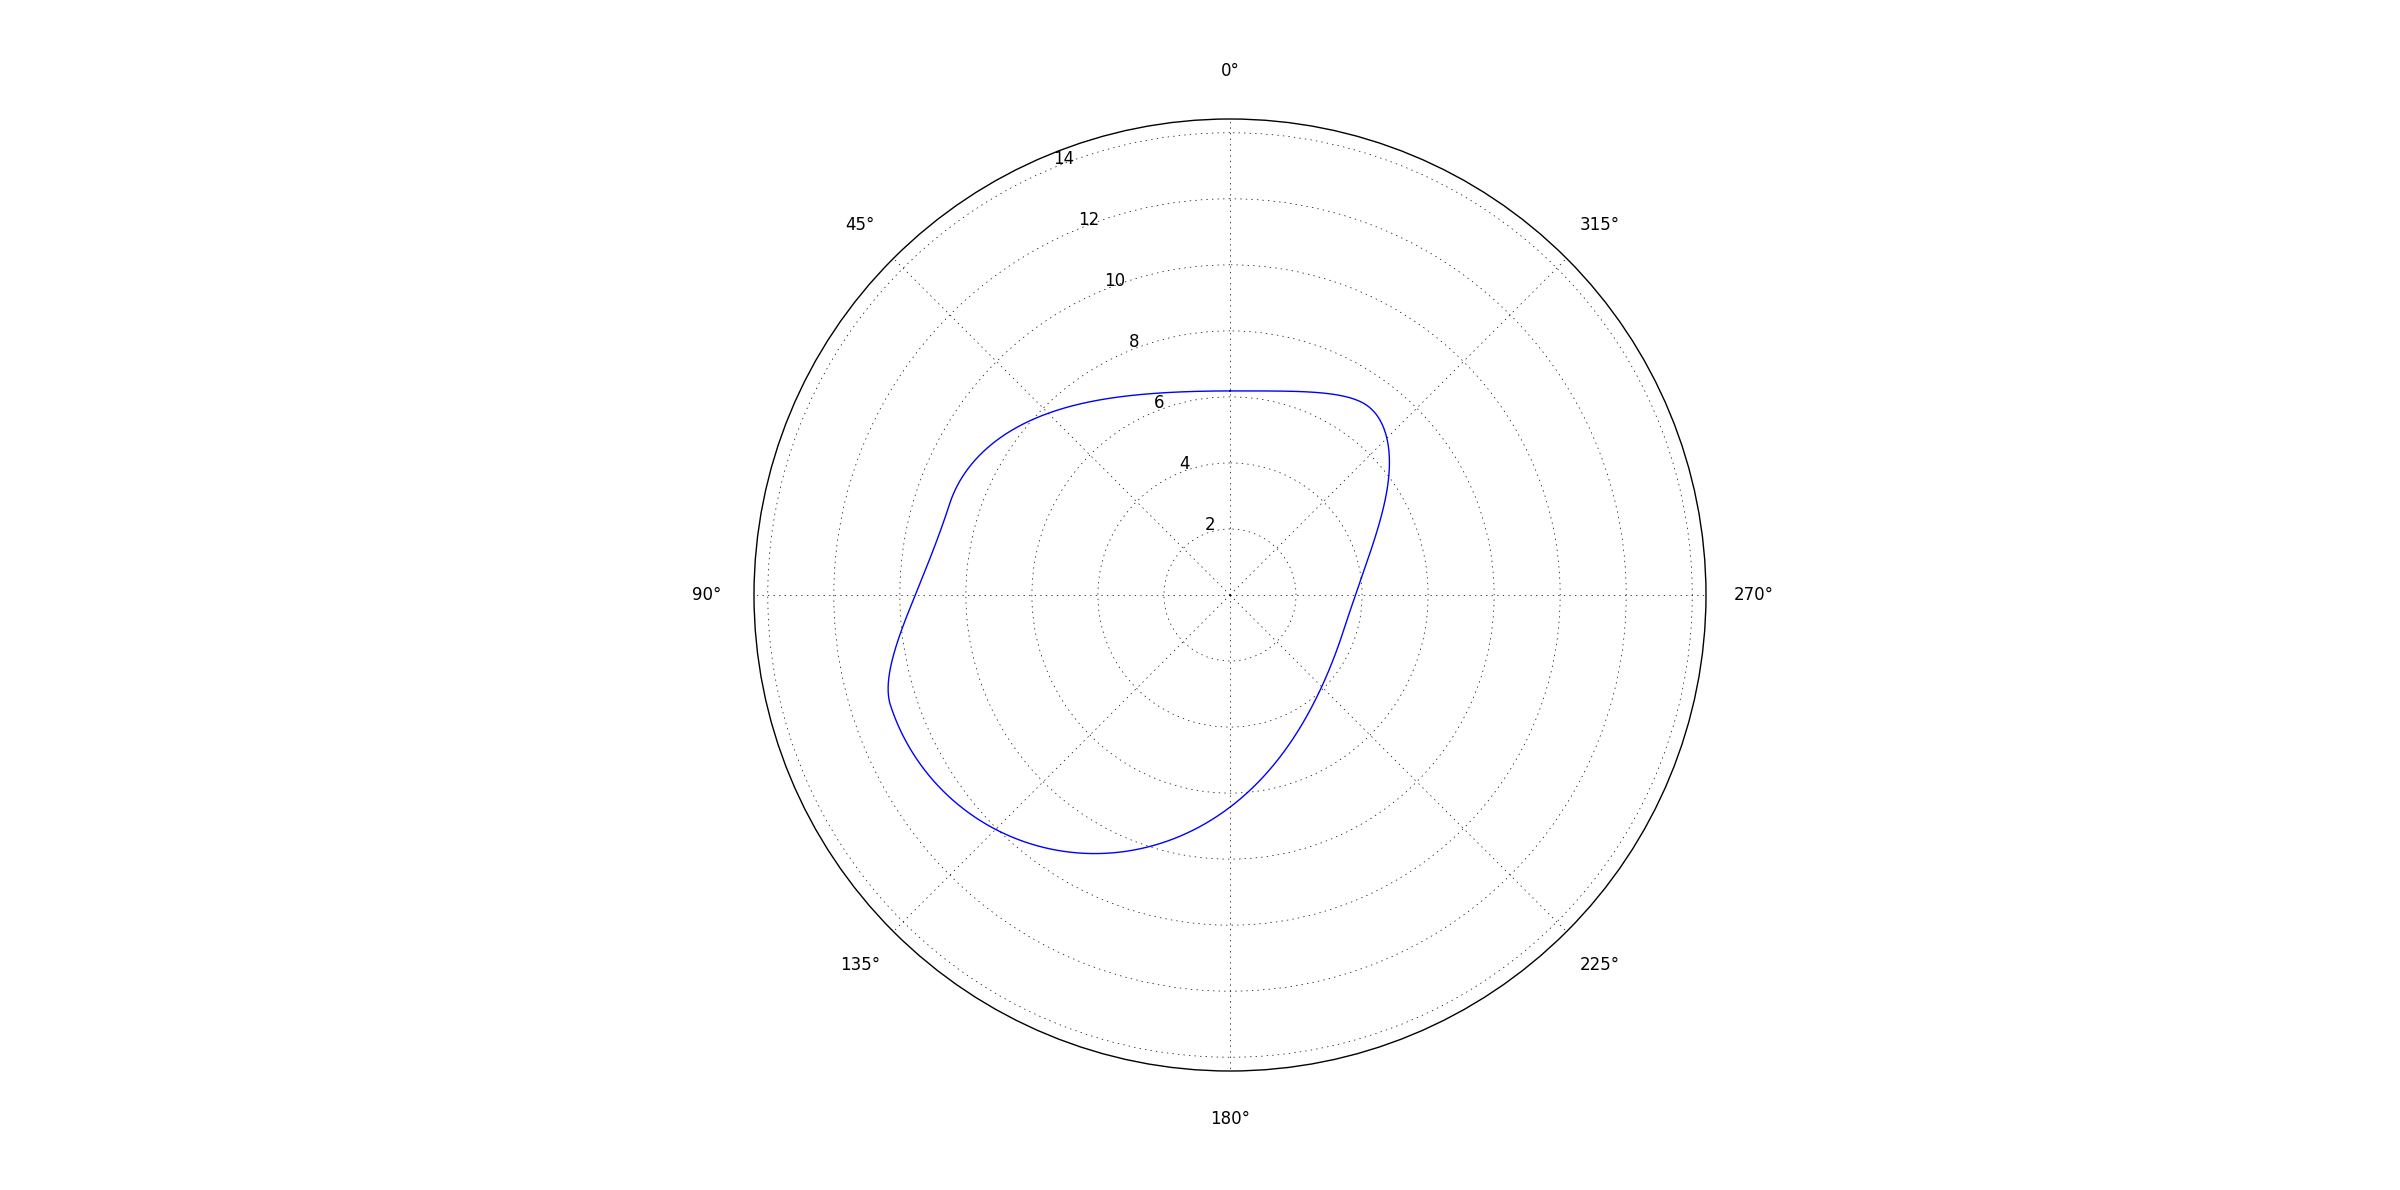
\includegraphics[width=\textwidth]{cam.png}

\section{Conjugated cam generation}
    \begin{verbatim}
    usage: gen conj [-h] [--breadth B]

    optional arguments:
      -h, --help            show this help message and exit
      --breadth B, -b B     breadth, if 0 calculate optimal (default)
    \end{verbatim}
The program is able to generate the constant-breadth conjugated cam. The breadth can be set or else it is used
the mean of cam diameters, an optimal value.
    \begin{pycode}
    def gen_conjugated(self, breadth=None):
        # For flat follower and others with diametrically opposed followers
        if breadth is None:
            breadth = self.breadth
        if breadth == 0:
            # Set breadth = mean cam diameter
            print('Searching optimal breadth')
            diam = self.pcoords[1] + self.interp(self.pcoords[0]+np.pi)
            breadth = diam.sum() / self.pcoords.shape[1]
        elif breadth < np.max(self.pcoords[1]):
            # maybe could be, with opposed values sum > 0
            raise HandledValueError('Breadth must be >= max radius ({:.3g})'
                                    .format(np.max(self.pcoords[1])))
        self.breadth = breadth
        print('Breadth:', breadth)
        self.conj_pcoords = np.empty_like(self.pcoords)
        for i in range(0, len(self.pcoords.T)):
            self.conj_pcoords[:, i] = (self.pcoords[0, i]+np.pi) % (2*np.pi),
                                       breadth - self.pcoords[1][i]
        # just fast, but probably a shift would be enough
        self.conj_pcoords = self.conj_pcoords[:, self.conj_pcoords[0].argsort()]
    \end{pycode}

    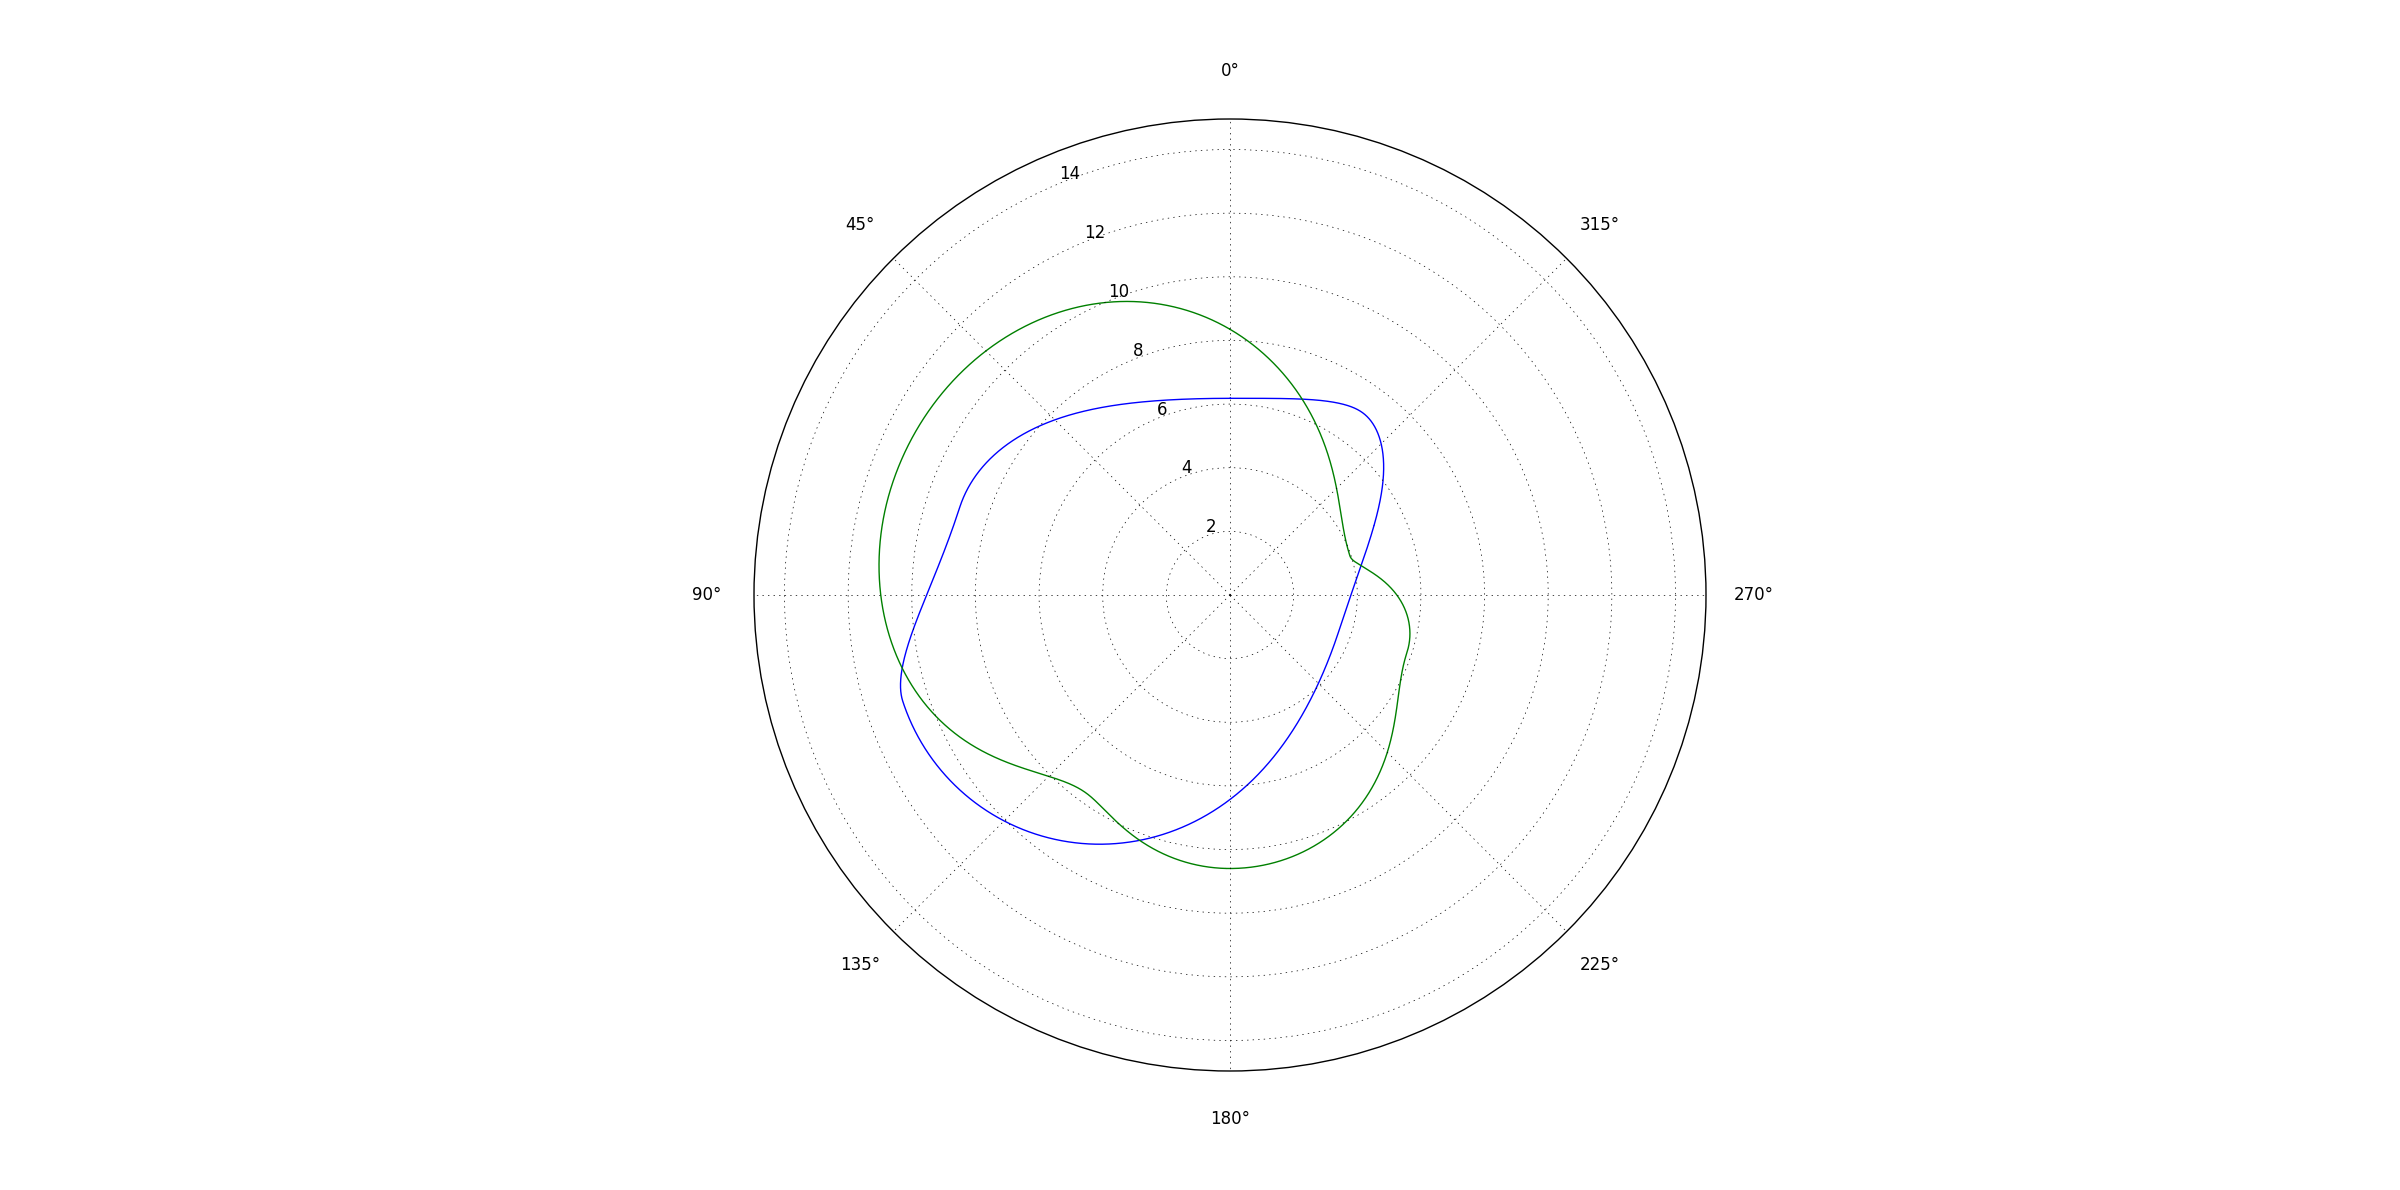
\includegraphics[width=\textwidth]{conj.png}

\section{STL exportation}\label{stl-exportation}
    \begin{verbatim}
    usage:  export [-h] file width

    positional arguments:
      file        output stl file
      width       cam width
    \end{verbatim}

    The 3-d model is a surface built with triangles. The program builds the 2-d face with Delaunay triangulation,
    then adds s third coordinate valued 0 to build the lower face, and valued \emph{width} for the upper face.
    \begin{pycode}
    # 2D Delaunay triangulation for front face and building of lower and upper faces
    tri0 = cam.points[Delaunay(cam.points).simplices]
    tri1 = np.concatenate((tri0, np.zeros([tri0.shape[0], tri0.shape[1], 1])), 2)
    tri2 = np.concatenate((tri0, np.ones([tri0.shape[0], tri0.shape[1], 1]) * width), 2)
    \end{pycode}

    Side surface is generated calculating each triangle's coordinates, which essentially links every couple of
    consecutive points of one face to a point on the other, as seen here:
    \begin{pycode}
    # Build triangles for side face
    vertices1 = np.concatenate((cam.points, np.zeros([cam.points.shape[0], 1])), 1)
    vertices2 = np.concatenate((cam.points, np.ones([cam.points.shape[0], 1]) * width), 1)
    tri3_1 = np.empty([cam.points.shape[0], 3, 3])
    tri3_2 = np.empty_like(tri3_1)
    for i in range(0, vertices1.shape[0]):
        tri3_1[i] = [vertices1[i-1], vertices1[i], vertices2[i]]
        tri3_2[i] = [vertices2[i-1], vertices2[i], vertices1[i-1]]
    \end{pycode}

    The program then concatenates the triangles and proceeds to save the model using methods from the \emph{stl} library.

\section{Simulation}\label{simulation}
    \begin{verbatim}
    usage:  sim [-h] [--omega W | --rpm RPM] [--steps S] [--precision P]
                [--gravity G]

    optional arguments:
      -h, --help           show this help message and exit
      --omega W, -w W      angular velocity (default: 1)
      --rpm RPM, -r RPM    revolutions per minute (default: None)
      --steps S, -s S      steps (default: 500)
      --precision P, -p P  precision (default: 0.001)
      --gravity G, -g G    gravitational acceleration (default: 9.8)
    \end{verbatim}

    The simulation is really basic and is just intended for visualization. The program draws the rotating cam and calculates
    the position of the follower. For flat follower the position is the maximum \emph{y} of the rotated cam
    \mintinline{python}{max(cam_coords[i][1])}.
    For knife follower it calculates the intersection of the cam with a
    vertical line at the follower offset and takes the upper \emph{y} bound
    \mintinline{python}{foll_body.intersection(cam_body).bounds[3]}.
    For roller follower the position is approximated, with given precision, with a bisection-like method.
    The first guess is found translating the follower with a constant step \emph{s} until the \emph{intersection state}
    changes, then halves \emph{s} and translates in the opposite direction.
    This ensure that the state changes between \emph{height-s} and \emph{height+s}.
    The precision is then improved with a bisection loop, translating and halving \emph{s} in each interarion.
    Finally the next height's first guess and \emph{s} are calculated with the finite differential.
    \begin{pycode}
    if foll_body.intersects(cam_body):
        translate(foll_body, yoff=s)
        height += s
        while foll_body.intersects(cam_body):
            translate(foll_body, yoff=s)
            height += s
        s /= 2
        translate(foll_body, yoff=-s)
        height -= s
    else:
        translate(foll_body, yoff=-s)
        height -= s
        while not foll_body.intersects(cam_body):
            translate(foll_body, yoff=-s)
            height -= s
        s /= 2
        translate(foll_body, yoff=+s)
        height += s
    s /= 2

    while s >= precision:
        if not foll_body.intersects(cam_body):
            translate(foll_body, yoff=-s)
            height -= s
        else:
            translate(foll_body, yoff=s)
            height += s
        s /= 2

    foll_heights[i] = height

    if i > 0:
        diff = height - foll_heights[i-1]
        height += diff
        translate(foll_body, yoff=diff)
        s = abs(diff) if diff != 0 else precision
    \end{pycode}

    Once all follower heights are determined the program calculates velocity and acceleration,
    then renders and displays the animation.

%\section{Utilities}\label{utilities}
%    \texttt{update} takes the same arguments as \texttt{gen} except for input file/function,
%    regenerate the target with update parameters (leaving immutated not explicit ones) and
%
%    \texttt{save} allows to store generated travel, cam or conjugated cam as CSVs,
%    for use or future reload with \texttt{load}.

https://github.com/fciotti/camdesign

\section{Source code}
\texttt{main.py}
\py{../main.py}

\texttt{fileio.py}
\py{../main.py}

\texttt{travel.py}
\py{../travel.py}

\texttt{follower.py}
\py{../follower.py}

\texttt{interpolation.py}
\py{../interpolation.py}

\texttt{cam.py}
\py{../cam.py}

\texttt{envelope.py}
\py{../envelope.py}

\texttt{export.py}
\py{../export.py}

\texttt{simulation.py}
\py{../simulation.py}

\texttt{utils.py}
\py{../utils.py}

\end{document}